\chapter{Asymptotics}

\begin{figure}[H]
    \centering
    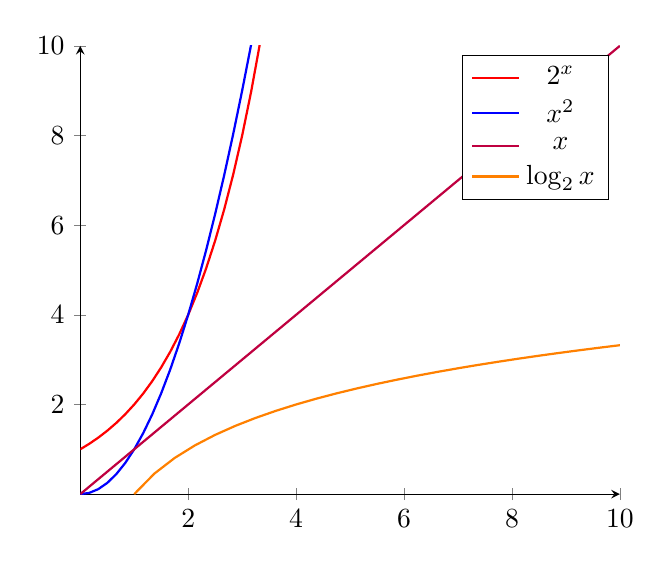
\begin{tikzpicture}
        \begin{axis}[axis lines = middle, xmin=0, xmax=10, ymin=0, ymax=10]
            \addplot[thick, color=red, domain=0:4]{2^(x)};
            \addplot[thick, color=blue, domain=0:4]{x^(2)};
            \addplot[thick, color=purple, domain=0:10]{x};
            \addplot[thick, color=orange, domain=1:10]{log2(x)};
            \addlegendentry{$2^x$};
            \addlegendentry{$x^2$};
            \addlegendentry{$x$};
            \addlegendentry{$\log_2{x}$};
        \end{axis}
    \end{tikzpicture}
    \caption{Comparison of the growth rate of various functions.}
    \label{fig:bigo_comparison}
\end{figure}

\begin{definition}
    The time complexity of an algorithm can be expressed in terms of the number of basic operations used by the algorithm when the input has a particular size.
    
    Examples of basic operations are
    \begin{enumerate}
        \item additions,
        \item multiplications,
        \item comparisons of two numbers, and
        \item swaps, assignments of values to variables.
    \end{enumerate}
\end{definition}

\begin{definition}
    The \textbf{space complexity} of an algorithm is expressed in terms of the memory required by the algorithm for an input of a particular size. 
\end{definition}

We will mainly be concerned with time complexity.

\begin{definition}
    The worst case time complexity of an algorithm can be expressed in terms of the largest number of basic operations used by the algorithm when the input has a particular case.
\end{definition}

Worst-case analysis tells us how many operations an algorithm requires to guarantee that it will produce a solution. The worst-case time analysis is a standard way to estimate the efficiency of algorithm. 

It is difficult to compute the exact number of operations. Usually, we don't need it. It is sufficient to estimate this number with bounds. We are interested in upper bounds for worst-case analysis. These bounds should give us the possibility to estimate growth of the number of operations when the input sizes increases.

\begin{remark}
    It is particularly important to estimate the number of operations when the input size is large.
\end{remark}

\section{Big-O}

\begin{definition}[Big-$O$]
Let $f, g : \mathbb R \to \mathbb R$. We say that $f(x) \in O(g(x))$ if \[ \exists \; k > 0 \; \exists \; N \in \mathbb R \; \forall \; n \geq N : \abs{f(n)} \leq k g(n), \] or equivalently \[ \limsup_{n \to \infty} \left( \frac{\abs{f(n)}}{g(n)} \right) < \infty. \]
\end{definition}

\begin{example}
    \begin{enumerate}
        \item Let $f(x)=x^2+2x+1$. Then $f(x) \in O(x^2)$.
            \begin{proof}
                For $x\geq 1$, we have $1\leq x\leq x^2$. That gives 
                \[f(x)=x^2+2x+1\leq x^2+2x^2+x^2=4x^2\] for $x\leq1$. Since the above inequality holds for $x\geq1$, using $k=1$ and $C=4$ as witnesses, we get \[f(x)\leq Cx^2\] for every $x\geq k$.
            \end{proof}
        \item Let $f(x)=3x^3-6x^2-4x+2$. For $x\geq1$,we have $1\leq x\leq x^2\leq x^3$. That gives $|f(x)|=|3x^3-7x^2-4x+2|\leq 3x^3 \implies f(x) \in O(x^3)$.
        \item Let $f(x)=3^x$. Then $f(x) \not \in O(2^x)$.
        \begin{proof}
            Assume that there are constants $k$ and $C$ such that $3^x\leq C2^x$ when $x\geq k$. Then, \[\left(\dfrac32\right)^x\leq C\] when $x\geq k$. But any exponential functions $a^x$ grows monotonically whenever $a\geq 1$; a contradiction.
        \end{proof}
        \item Let $a,b>1$. Then $\log_a{x}\in O(\log_b{x})$.
        \begin{proof}
            We know that \[\log_a{x}=\dfrac{\log_b{x}}{\log_b{a}},\] hence, we can take \[C=\dfrac{1}{\log_b{a}}\] and any $k>0$.
        \end{proof}
        \item Let $0<p<q$. Then $x^p\in O(x^q)$ but $x^q \not \in O(x^p)$. 
        \begin{proof}
            For any $x\geq 1$, $x^p\leq x^q$. Hence we can take $C=1$ and $k=1$, Assume there are constants $k$ and $C$ such that $x^q\leq Cx^p$ when $x\geq k$. Then \[x^{q-p}\leq C.\] Observe that $r=q-p>0$. Any function $x^r$ grows monotonically whenever $r>0$; a contradiction.
        \end{proof}
        \item Let $a>1$ and let $0<p$. Then $x^p\in O(a^x)$ but $a^x$ is not $O(x^p)$.
        \item Let $a>1$ and let $0<p$. Then $\log_a{x}\in O(x^p)$ but $x^p$ is not $O(log_a{x})$.
    \end{enumerate}
\end{example}

\begin{theorem}[The sum rule]
    Let $f_1(x) \in O(g_1(x))$ and $f_2(x) \in O(g_2(x))$. Then \[ f_1(x)+f_2(x) \in O(g_1) \cup O(g_2). \]
\end{theorem}

\begin{proof}
    Let $C_i$ and $k_i$ be witness pairs for $f_i(x)$ is $O(g_i(x))$, for $i=1,2$.
    
    Let $k=\max\{k_1,k_2\}$ and $C=C_1+C_2$. Then for $x>k$ we have $|f_1(x)+f_2(x)|\leq|f_1(x)|+|f_2(x)|\leq C_1|g_1(x)|+C_2|g_2(x)|$
\end{proof}

\begin{theorem}[The product rule]
    Let $f_1(x) \in O(g_1(x))$ and $f_2(x) \in O(g_2(x))$. Then \[ f_1(x)f_2(x) \in O(g_1(x)g_2(x)). \]
\end{theorem}

\begin{proof}
    Let $C_i$ and $k_i$ be witness pairs for $f_i(x)$ is $O(g_i(x))$, for $i = 1, 2$. Let $k=\max\{ k_1, k_2 \}$ and $C = C_1 C_2$. Then for $x > k$ we have \[ \abs{f_1(x) f_2(x)} = \abs{f_1(x) f_2(x)} \leq  C_1 \abs{g_1(x)} C_2 \abs{g_2(x)} = C \abs{g_1(x) g_2(x)}. \]
\end{proof}

\begin{proposition}
    Let $a_0,a_1,\ldots,a_n$ be real numbers and \[f(x)=a_nx^n+a_{n-1}x^{n-1}+\ldots+a_1x+a_0.\] Then $f(x)\in O(x^n)$.
\end{proposition}

\begin{proof}
    For each $0\leq k\leq n$, $x^k\in O(x^n)$.
    
    Then we observe that for any constant $a$, $ax^k\in O(x^n)$. By the sum rule $f(x)\in O(x^n)$.
\end{proof}

\section{Big-Omega}

The BigO notation is very useful to find reasonable upper bounds for growth rates, but does not really help miuch if we are intersested in the best function that matches the growth rate.

AS a first step in thisdirection, we introduce a similar definition for lower bounds which is called Big-Omega notation.

\begin{definition}[Big-$\Omega$]
    Let $f, g : \mathbb R \to \mathbb R$. We say that $f(x) \in \Omega(g(x))$ if \[ \exists \; k > 0 \; \exists \; N \in \mathbb N \; \forall \; n > N : \abs{f(n)} \geq k g(n). \]
\end{definition}

\begin{remark}
    Note that the previous definition implies that $f(x)$ is $\Omega g(x)$ if and only if $g(x)$ is $O(f(x))$.
\end{remark}

\section{Theta}

\begin{definition}[$\Theta$]
    Let $f, g : \mathbb R \to \mathbb R$. We say that $f(x) \in \Theta(g(x))$ if $f(x) \in O(g(x)$ and $g(x) \in O(f(x))$.
\end{definition}

This is equivalent to saying that $f(x)$ is $\Theta(g(x))$ if $f(x)$ is $O(g(x))$ and $g(x)$ is $O(f(x))$.

And this is equivalent to saying that there are constants $C_1,C_2,k$ such that $|f(x)|\leq C_1\|g(x)|$ and $|g(x)|\leq C_2|f(x)|$ whenever $x\geq k$.

\begin{example}
    All polynomials of order greater than $n>0$ are $\Theta(x^n)$.
\end{example}

\section{Little-$o$}



\begin{definition}[Little-$o$]
    Let $f(x)$ and $g(x)$ be functions from the set of real numbers to the set of real numbers. We say that $f(x)$ is $o(g(x))$, (little-$o$ of $g(x)$) when \[\lim_{x\to\infty}\dfrac{f(x)}{g(x)}=0.\]
    Formally,
    \[o(g)=\{f:\mathbb N\mapsto\mathbb N:\forall\; C>0\;\exists\;k>0:Cf(n)<g(n)\;\forall\;n\geq k\}\]
    More informally, this means that $g(x)$ grows much faster than $f(x)$.
\end{definition}


\begin{definition}
    A function $f(x)$ is called sublinear if $f(x)$ is $o(x)$, so if \[\lim_{n\to\infty}\dfrac{f(x)}{x}=0.\]
\end{definition}

\begin{example}
    \[f(x)=\dfrac{100x}{\log{x}}\] is sublinear since \[\lim_{n\to\infty}\left(\dfrac{f(x)}{x}\right)=\lim_{n\to\infty}\left(\dfrac{100}{\log{x}}\right)=0.\]
\end{example}

\begin{definition}[Small-$\omega$]
    \[\omega(g)=\{f:\mathbb N\mapsto \mathbb N:\forall\; C>0\;\exists\;k>0:f(n)>Cg(n)\;\forall\;n\geq k\}\]
\end{definition}

\begin{theorem}
    If $f_1(x)$ is $o(g(x))$ and $f_2(x)$ is $o(g(x))$, then $f_1(x)+f_2(x)$ is $o(g(x))$.
\end{theorem}

\begin{theorem}
    If $f_1(x)$ is $O(g(x))$ and $f_2(x)$ is $o(g(x))$, then $f_1(x)+f_2(x)$ is $O(g(x))$.
\end{theorem}

\begin{theorem}
    If $f_1(x)$ is $\Theta(g(x))$ and $f_2(x)$ is $o(g(x))$, then $f_1(x)+f_2(x)$ is $\Theta(g(x))$.
\end{theorem}
